\documentclass[11pt,compress,t,notes=noshow, xcolor=table]{beamer}
\usepackage[]{graphicx}
% graphicx is loaded via lmu-lecture.sty as well
\usepackage[]{color}
% maxwidth is the original width if it is less than linewidth
% otherwise use linewidth (to make sure the graphics do not exceed the margin)
\makeatletter
\def\maxwidth{ %
  \ifdim\Gin@nat@width>\linewidth
    \linewidth
  \else
    \Gin@nat@width
  \fi
}
\makeatother

% ---------------------------------%
% latex-math dependencies, do not remove:
% - mathtools
% - bm
% - siunitx
% - dsfont
% - xspace
% ---------------------------------%

%--------------------------------------------------------%
%       Language, encoding, typography
%--------------------------------------------------------%

\usepackage[english]{babel}
\usepackage[utf8]{inputenc} % Enables inputting UTF-8 symbols
% Standard AMS suite (loaded via lmu-lecture.sty)
\usepackage{amsmath,amsfonts,amssymb}

% Font for double-stroke / blackboard letters for sets of numbers (N, R, ...)
% Distribution name is "doublestroke"
% According to https://mirror.physik.tu-berlin.de/pub/CTAN/fonts/doublestroke/dsdoc.pdf
% the "bbm" package does a similar thing and may be superfluous.
% Required for latex-math
\usepackage{dsfont}

% bbm – "Blackboard-style" cm fonts (https://www.ctan.org/pkg/bbm)
% Used to be in common.tex, loaded directly after this file
% Maybe superfluous given dsfont is loaded
% TODO: Check if really unused?
% \usepackage{bbm}

% bm – Access bold symbols in maths mode - https://ctan.org/pkg/bm
% Required for latex-math, preferred over \boldsymbol
% https://tex.stackexchange.com/questions/3238/bm-package-versus-boldsymbol
\usepackage{bm}

% pifont – Access to PostScript standard Symbol and Dingbats fonts
% Used for \newcommand{\xmark}{\ding{55}, which is never used
% aside from lecture_advml/attic/xx-automl/slides.Rnw
% \usepackage{pifont}

% Quotes (inline and display), provdes \enquote
% https://ctan.org/pkg/csquotes
\usepackage{csquotes}

% Adds arg to enumerate env, technically superseded by enumitem according
% to https://ctan.org/pkg/enumerate
% Replace with https://ctan.org/pkg/enumitem ?
% Even better: enumitem is not really compatible with beamer and breaks all sorts of things
% particularly the enumerate environment. The enumerate package also just isn't required
% from what I can tell so... don't re-add it I guess?
% \usepackage{enumerate}

% Line spacing - provides \singlespacing \doublespacing \onehalfspacing
% https://ctan.org/pkg/setspace
% \usepackage{setspace}

% mathtools – Mathematical tools to use with amsmath
% https://ctan.org/pkg/mathtools?lang=en
% latex-math dependency according to latex-math repo
\usepackage{mathtools}

% Maybe not great to use this https://tex.stackexchange.com/a/197/19093
% Use align instead -- TODO: Global search & replace to check, eqnarray is used a lot
% $ rg -f -u "\begin{eqnarray" -l | grep -v attic | awk -F '/' '{print $1}' | sort | uniq -c
%   13 lecture_advml
%   14 lecture_i2ml
%    2 lecture_iml
%   27 lecture_optimization
%   45 lecture_sl
\usepackage{eqnarray}

% For shaded regions / boxes
% Used sometimes in optim
% https://www.ctan.org/pkg/framed
\usepackage{framed}

%--------------------------------------------------------%
%       Cite button (version 2024-05)
%--------------------------------------------------------%

% Superseded by style/ref-buttons.sty, kept just in case these don't work out somehow.

% Note this requires biber to be in $PATH when running,
% telltale error in log would be e.g. Package biblatex Info: ... file 'authoryear.dbx' not found
% aside from obvious "biber: command not found" or similar.
% Tried moving this to lmu-lecture.sty but had issues I didn't quite understood,
% so it's here for now.

\usepackage{textcase} % for \NoCaseChange
\usepackage{hyperref}

% Only try adding a references file if it exists, otherwise
% this would compile error when references.bib is not found
% NOTE: Bibliography packages (usebib, biblatex) are now loaded by ref-buttons.sty when needed
% This keeps all bibliography-related setup in one place

% \newcommand{\citelink}[1]{%
% \NoCaseChange{\resizebox{!}{9pt}{\protect\beamergotobutton{\href{\usebibentry{\NoCaseChange{#1}}{url}}{\begin{NoHyper}\cite{#1}\end{NoHyper}}}}}%
% }

%--------------------------------------------------------%
%       Displaying code and algorithms
%--------------------------------------------------------%

% Reimplements verbatim environments: https://ctan.org/pkg/verbatim
% verbatim used sed at least once in
% supervised-classification/slides-classification-tasks.tex
% Removed since code should not be put on slides anyway
% \usepackage{verbatim}

% Both used together for algorithm typesetting, see also overleaf: https://www.overleaf.com/learn/latex/Algorithms
% algorithmic env is also used, but part of the bundle:
%   "algpseudocode is part of the algorithmicx bundle, it gives you an improved version of algorithmic besides providing some other features"
% According to https://tex.stackexchange.com/questions/229355/algorithm-algorithmic-algorithmicx-algorithm2e-algpseudocode-confused
\usepackage{algorithm}
\usepackage{algpseudocode}

%--------------------------------------------------------%
%       Tables
%--------------------------------------------------------%

% multi-row table cells: https://www.namsu.de/Extra/pakete/Multirow.html
% Provides \multirow
% Used e.g. in evaluation/slides-evaluation-measures-classification.tex
\usepackage{multirow}

% colortbl: https://ctan.org/pkg/colortbl
% "The package allows rows and columns to be coloured, and even individual cells." well.
% Provides \columncolor and \rowcolor
% \rowcolor is used multiple times, e.g. in knn/slides-knn.tex
\usepackage{colortbl}

% long/multi-page tables: https://texdoc.org/serve/longtable.pdf/0
% Not used in slides
% \usepackage{longtable}

% pretty table env: https://ctan.org/pkg/booktabs
% Is used
% Defines \toprule
\usepackage{booktabs}

%--------------------------------------------------------%
%       Figures: Creating, placing, verbing
%--------------------------------------------------------%

% wrapfig - Wrapping text around figures https://de.overleaf.com/learn/latex/Wrapping_text_around_figures
% Provides wrapfigure environment -used in lecture_optimization
\usepackage{wrapfig}

% Sub figures in figures and tables
% https://ctan.org/pkg/subfig -- supersedes subfigure package
% Provides \subfigure
% \subfigure not used in slides but slides-tuning-practical.pdf errors without this pkg, error due to \captionsetup undefined
\usepackage{subfig}

% Actually it's pronounced PGF https://en.wikibooks.org/wiki/LaTeX/PGF/TikZ
\usepackage{tikz}

% No idea what/why these settings are what they are but I assume they're there on purpose
\usetikzlibrary{shapes,arrows,automata,positioning,calc,chains,trees, shadows}
\tikzset{
  %Define standard arrow tip
  >=stealth',
  %Define style for boxes
  punkt/.style={
    rectangle,
    rounded corners,
    draw=black, very thick,
    text width=6.5em,
    minimum height=2em,
    text centered},
  % Define arrow style
  pil/.style={
    ->,
    thick,
    shorten <=2pt,
    shorten >=2pt,}
}

%--------------------------------------------------------%
%       Beamer setup and custom macros & environments
%--------------------------------------------------------%

% Main sty file for beamer setup (layout, style, lecture page numbering, etc.)
% For long-term maintenance, this may me refactored into a more modular set of .sty files
\usepackage{../../style/lmu-lecture}
% Custom itemize wrappers, itemizeS, itemizeL, etc
\usepackage{../../style/customitemize}
% Custom framei environment, uses custom itemize!
\usepackage{../../style/framei}
% Custom frame2 environment, allows specifying font size for all content
\usepackage{../../style/frame2}
% Column layout macros
\usepackage{../../style/splitV}
% \image and derivatives
\usepackage{../../style/image}
% New generation of reference button macros
\usepackage{../../style/ref-buttons}

% Used regularly
\let\code=\texttt

% Not sure what/why this does
\setkeys{Gin}{width=0.9\textwidth}

% -- knitr leftovers --
% Used often in conjunction with \definecolor{shadecolor}{rgb}{0.969, 0.969, 0.969}
% Removing definitions requires chaning _many many_ slides, which then need checking to see if output still ok
\definecolor{fgcolor}{rgb}{0.345, 0.345, 0.345}
\definecolor{shadecolor}{rgb}{0.969, 0.969, 0.969}
\newenvironment{knitrout}{}{} % an empty environment to be redefined in TeX

%-------------------------------------------------------------------------------------------------------%
%  Unused stuff that needs to go but is kept here currently juuuust in case it was important after all  %
%-------------------------------------------------------------------------------------------------------%

% \newcommand{\hlnum}[1]{\textcolor[rgb]{0.686,0.059,0.569}{#1}}%
% \newcommand{\hlstr}[1]{\textcolor[rgb]{0.192,0.494,0.8}{#1}}%
% \newcommand{\hlcom}[1]{\textcolor[rgb]{0.678,0.584,0.686}{\textit{#1}}}%
% \newcommand{\hlopt}[1]{\textcolor[rgb]{0,0,0}{#1}}%
% \newcommand{\hlstd}[1]{\textcolor[rgb]{0.345,0.345,0.345}{#1}}%
% \newcommand{\hlkwa}[1]{\textcolor[rgb]{0.161,0.373,0.58}{\textbf{#1}}}%
% \newcommand{\hlkwb}[1]{\textcolor[rgb]{0.69,0.353,0.396}{#1}}%
% \newcommand{\hlkwc}[1]{\textcolor[rgb]{0.333,0.667,0.333}{#1}}%
% \newcommand{\hlkwd}[1]{\textcolor[rgb]{0.737,0.353,0.396}{\textbf{#1}}}%
% \let\hlipl\hlkwb

% \makeatletter
% \newenvironment{kframe}{%
%  \def\at@end@of@kframe{}%
%  \ifinner\ifhmode%
%   \def\at@end@of@kframe{\end{minipage}}%
%   \begin{minipage}{\columnwidth}%
%  \fi\fi%
%  \def\FrameCommand##1{\hskip\@totalleftmargin \hskip-\fboxsep
%  \colorbox{shadecolor}{##1}\hskip-\fboxsep
%      % There is no \\@totalrightmargin, so:
%      \hskip-\linewidth \hskip-\@totalleftmargin \hskip\columnwidth}%
%  \MakeFramed {\advance\hsize-\width
%    \@totalleftmargin\z@ \linewidth\hsize
%    \@setminipage}}%
%  {\par\unskip\endMakeFramed%
%  \at@end@of@kframe}
% \makeatother

% \definecolor{shadecolor}{rgb}{.97, .97, .97}
% \definecolor{messagecolor}{rgb}{0, 0, 0}
% \definecolor{warningcolor}{rgb}{1, 0, 1}
% \definecolor{errorcolor}{rgb}{1, 0, 0}
% \newenvironment{knitrout}{}{} % an empty environment to be redefined in TeX

% \usepackage{alltt}
% \newcommand{\SweaveOpts}[1]{}  % do not interfere with LaTeX
% \newcommand{\SweaveInput}[1]{} % because they are not real TeX commands
% \newcommand{\Sexpr}[1]{}       % will only be parsed by R
% \newcommand{\xmark}{\ding{55}}%

% textpos – Place boxes at arbitrary positions on the LATEX page
% https://ctan.org/pkg/textpos
% Provides \begin{textblock}
% TODO: Check if really unused?
% \usepackage[absolute,overlay]{textpos}

% -----------------------%
% Likely knitr leftovers %
% -----------------------%

% psfrag – Replace strings in encapsulated PostScript figures
% https://www.overleaf.com/latex/examples/psfrag-example/tggxhgzwrzhn
% https://ftp.mpi-inf.mpg.de/pub/tex/mirror/ftp.dante.de/pub/tex/macros/latex/contrib/psfrag/pfgguide.pdf
% Can't tell if this is needed
% TODO: Check if really unused?
% \usepackage{psfrag}

% arydshln – Draw dash-lines in array/tabular
% https://www.ctan.org/pkg/arydshln
% !! "arydshln has to be loaded after array, longtable, colortab and/or colortbl"
% Provides \hdashline and \cdashline
% Not used in slides
% \usepackage{arydshln}

% tabularx – Tabulars with adjustable-width columns
% https://ctan.org/pkg/tabularx
% Provides \begin{tabularx}
% Not used in slides
% \usepackage{tabularx}

% placeins – Control float placement
% https://ctan.org/pkg/placeins
% Defines a \FloatBarrier command
% TODO: Check if really unused?
% \usepackage{placeins}

% Can't find a reason why common.tex is not just part of this file?
% This file is included in slides and exercises

% Rarely used fontstyle for R packages, used only in 
% - forests/slides-forests-benchmark.tex
% - exercises/single-exercises/methods_l_1.Rnw
% - slides/cart/attic/slides_extra_trees.Rnw
\newcommand{\pkg}[1]{{\fontseries{b}\selectfont #1}}

% Spacing helpers, used often (mostly in exercises for \dlz)
\newcommand{\lz}{\vspace{0.5cm}} % vertical space (used often in slides)
\newcommand{\dlz}{\vspace{1cm}}  % double vertical space (used often in exercises, never in slides)
\newcommand{\oneliner}[1] % Oneliner for important statements, used e.g. in iml, algods
{\begin{block}{}\begin{center}\begin{Large}#1\end{Large}\end{center}\end{block}}

% Don't know if this is used or needed, remove?
% textcolor that works in mathmode
% https://tex.stackexchange.com/a/261480
% Used e.g. in forests/slides-forests-bagging.tex
% [...] \textcolor{blue}{\tfrac{1}{M}\sum^M_{m} [...]
% \makeatletter
% \renewcommand*{\@textcolor}[3]{%
%   \protect\leavevmode
%   \begingroup
%     \color#1{#2}#3%
%   \endgroup
% }
% \makeatother


% dependencies: amsmath, amssymb, dsfont
% math spaces
\ifdefined\N
\renewcommand{\N}{\mathds{N}} % N, naturals
\else \newcommand{\N}{\mathds{N}} \fi
\newcommand{\Z}{\mathds{Z}} % Z, integers
\newcommand{\Q}{\mathds{Q}} % Q, rationals
\newcommand{\R}{\mathds{R}} % R, reals
\ifdefined\C
\renewcommand{\C}{\mathds{C}} % C, complex
\else \newcommand{\C}{\mathds{C}} \fi
\newcommand{\continuous}{\mathcal{C}} % C, space of continuous functions
\newcommand{\M}{\mathcal{M}} % machine numbers
\newcommand{\epsm}{\epsilon_m} % maximum error

% counting / finite sets
\newcommand{\setzo}{\{0, 1\}} % set 0, 1
\newcommand{\setmp}{\{-1, +1\}} % set -1, 1
\newcommand{\unitint}{[0, 1]} % unit interval

% basic math stuff
\newcommand{\xt}{\tilde x} % x tilde
\newcommand{\argmin}{\mathop{\mathrm{arg\,min}}} % argmin
\newcommand{\argmax}{\mathop{\mathrm{arg\,max}}} % argmax
\newcommand{\argminlim}{\argmin\limits} % argmin with limits
\newcommand{\argmaxlim}{\argmax\limits} % argmax with limits
\newcommand{\sign}{\operatorname{sign}} % sign, signum
\newcommand{\I}{\mathbb{I}} % I, indicator
\newcommand{\order}{\mathcal{O}} % O, order
\newcommand{\bigO}{\mathcal{O}} % Big-O Landau
\newcommand{\littleo}{{o}} % Little-o Landau
\newcommand{\pd}[2]{\frac{\partial{#1}}{\partial #2}} % partial derivative
\newcommand{\floorlr}[1]{\left\lfloor #1 \right\rfloor} % floor
\newcommand{\ceillr}[1]{\left\lceil #1 \right\rceil} % ceiling
\newcommand{\indep}{\perp \!\!\! \perp} % independence symbol

% sums and products
\newcommand{\sumin}{\sum\limits_{i=1}^n} % summation from i=1 to n
\newcommand{\sumim}{\sum\limits_{i=1}^m} % summation from i=1 to m
\newcommand{\sumjn}{\sum\limits_{j=1}^n} % summation from j=1 to p
\newcommand{\sumjp}{\sum\limits_{j=1}^p} % summation from j=1 to p
\newcommand{\sumik}{\sum\limits_{i=1}^k} % summation from i=1 to k
\newcommand{\sumkg}{\sum\limits_{k=1}^g} % summation from k=1 to g
\newcommand{\sumjg}{\sum\limits_{j=1}^g} % summation from j=1 to g
\newcommand{\summM}{\sum\limits_{m=1}^M} % summation from m=1 to M
\newcommand{\meanin}{\frac{1}{n} \sum\limits_{i=1}^n} % mean from i=1 to n
\newcommand{\meanim}{\frac{1}{m} \sum\limits_{i=1}^m} % mean from i=1 to n
\newcommand{\meankg}{\frac{1}{g} \sum\limits_{k=1}^g} % mean from k=1 to g
\newcommand{\meanmM}{\frac{1}{M} \sum\limits_{m=1}^M} % mean from m=1 to M
\newcommand{\prodin}{\prod\limits_{i=1}^n} % product from i=1 to n
\newcommand{\prodkg}{\prod\limits_{k=1}^g} % product from k=1 to g
\newcommand{\prodjp}{\prod\limits_{j=1}^p} % product from j=1 to p

% linear algebra
\newcommand{\one}{\bm{1}} % 1, unitvector
\newcommand{\zero}{\mathbf{0}} % 0-vector
\newcommand{\id}{\bm{I}} % I, identity
\newcommand{\diag}{\operatorname{diag}} % diag, diagonal
\newcommand{\trace}{\operatorname{tr}} % tr, trace
\newcommand{\spn}{\operatorname{span}} % span
\newcommand{\scp}[2]{\left\langle #1, #2 \right\rangle} % <.,.>, scalarproduct
\newcommand{\mat}[1]{\begin{pmatrix} #1 \end{pmatrix}} % short pmatrix command
\newcommand{\Amat}{\mathbf{A}} % matrix A
\newcommand{\Deltab}{\mathbf{\Delta}} % error term for vectors

% basic probability + stats
\renewcommand{\P}{\mathds{P}} % P, probability
\newcommand{\E}{\mathds{E}} % E, expectation
\newcommand{\var}{\mathsf{Var}} % Var, variance
\newcommand{\cov}{\mathsf{Cov}} % Cov, covariance
\newcommand{\corr}{\mathsf{Corr}} % Corr, correlation
\newcommand{\normal}{\mathcal{N}} % N of the normal distribution
\newcommand{\iid}{\overset{i.i.d}{\sim}} % dist with i.i.d superscript
\newcommand{\distas}[1]{\overset{#1}{\sim}} % ... is distributed as ...


\title{Introduction to Debugging Lectures}

\begin{document}

\titlemeta{% Chunk title (example: CART, Forests, Boosting, ...), can be empty
Demo Lecture
}{% Lecture title  
Layout Macro Testing With Cannibalized Content
}{% Relative path to title page image: Can be empty but must not start with slides/
figure/compboost-illustration-2.png
}{
\item Test layout
\item Fix stuff
\item Go home
}
% ------------------------------------------------------------------------------

\begin{frame}{Demo Slides}
  This is a demo lecture chunk.
  
  It is recommended to view these slides as PDF and LaTeX code side by side
  
  Refer to the \code{slds-lmu/lecture\_debug} repository for the source and PDF:
  \begin{itemizeS}
    \item \href{https://slds-lmu.github.io/lecture_debug/lecture_debug/slides/demo/slides-demo-layout.pdf}{\beamergotobutton{Compiled PDF}}
    \item \href{https://github.com/slds-lmu/lecture_debug/blob/main/slides/demo/slides-demo-layout.tex}{\beamergotobutton{LaTeX source}}
  \end{itemizeS}
  
\end{frame}

\begin{frame}{\textbackslash splitV(TCB)(TCB)}
  
  \begin{itemize}
    \item \code{\textbackslash splitVCC} creates two centered columns
    \item \code{\textbackslash splitVTT} creates two top-aligned columns 
    \item \code{\textbackslash splitVBB} for bottom-aligned columns
  \end{itemize}
  
  \vfill
  
  \splitVTT{
  \textbf{Left column} these two columns should both be top-aligned with their unequal content lengths
  }{
  \textbf{Right column} Lorem ipsum dolor sit amet, consectetur adipiscing elit
  }
  
  \vfill
  
  \splitVCC{
  \begin{itemize}
    \item Example itemize content for centered columns
    \item Second itemize item
  \end{itemize}
  }{
  Lorem ipsum dolor sit amet, consectetur adipiscing elit
  }
  
\end{frame}

% ------------------------------------------------------------------------------

\begin{frame}{\textbackslash splitV with unequal sizes}
  
  You only need to specify the width of the first column:
  
  \vfill
  
  \code{\textbackslash splitVTT[0.75]\{left content\}\{right content\}} creates a column with 75\% width and the
  second column will fill the remaining space:
  
  \vfill
  
  \splitVTT[0.75]{First column with 75\% of the text width on the slide}{Second column with rest}
  
  \vfill
  
  \splitVTT[0.2]{Tiny column}{Second column with a lot of room for activities}
  
\end{frame}

% ------------------------------------------------------------------------------

\begin{frame}{Two columns, minimal adjustments}
  
  Compact version if you do not want to use the full slide width:
  
  \code{\textbackslash splitVCompact\{0.2\}\{0.2\}} only takes up 20\% of the slide width in each column for a total of 40\% with a minimal horizontal spacer:
  
  \vfill
  
  \splitVCompact{0.20}{0.20}{First column with 20\%}{Second column with 20\%}
  
  
\end{frame}

% ------------------------------------------------------------------------------

\begin{frame}{3 columns}
  
  Using \code{\textbackslash splitVThree\{Left\}\{Middle\}\{Right\}} for 3 equally sized columns:
  
  \vfill
  
  \splitVThree{
  First column content is here
  }{
  Second column content is here as well
  }{
  And also a third column is here just in case
  }
  
  \vfill
  
  Then there is \code{\textbackslash splitVThreeCustom} for three columns of
  arbitrary widths, where the width of the third column can also be inferred from the first two
  \vfill
  
  \splitVThreeCustom[0.2]{0.2}{0}{
  first column with 20\% width
  }{
  second column with 20\% width
  }{
  third column with remaining width
  }
  
\end{frame}

% ------------------------------------------------------------------------------

\begin{frame}{twobytwo 2$\times$2 layout / quadrants}
  
  Use \code{\textbackslash twobytwo\{top left\}\{top  right\}\{bottom left\}\{bottom right\}} for horizontally aligned quadrants
  
  \vfill
  
  \twobytwo{%
  \begin{itemize}
    \item Example top left...
    \item ...quadrant content
    \item Next to a figure
  \end{itemize}
  }{%
  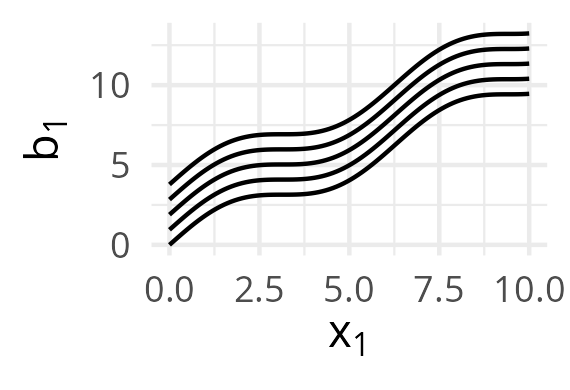
\includegraphics[width=\textwidth]{figure/boosting-cwb-blpool1.png}
  }{%
  \begin{itemize}
    \item Bottom left...
    \item ...quadrant content
  \end{itemize}
  }{%
  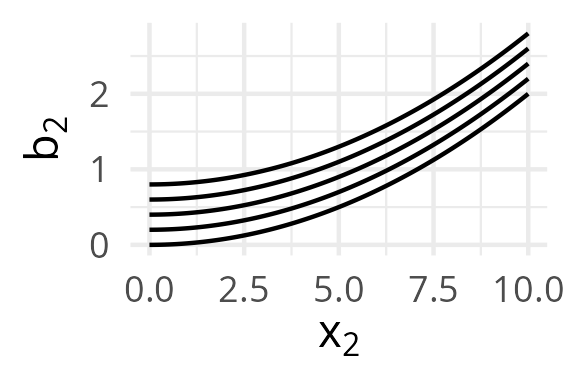
\includegraphics[width=\textwidth]{figure/boosting-cwb-blpool2.png}
  }
  
\end{frame}

% ------------------------------------------------------------------------------

\begin{frame}{2$\times$2 layout: All images}
  
  \vfill
  
  \twobytwo{%
  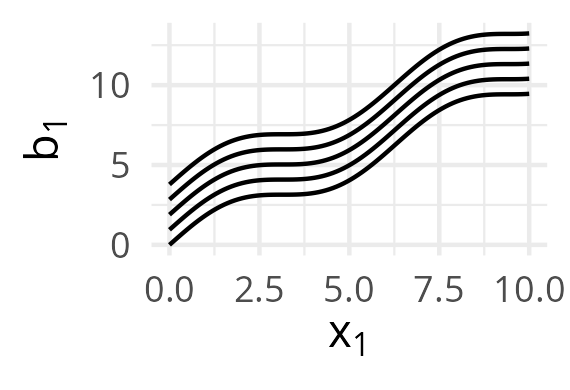
\includegraphics[width=\textwidth]{figure/boosting-cwb-blpool1.png}
  }{%
  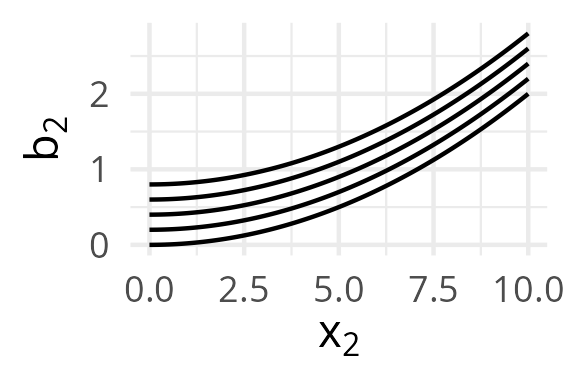
\includegraphics[width=\textwidth]{figure/boosting-cwb-blpool2.png}
  }{%
  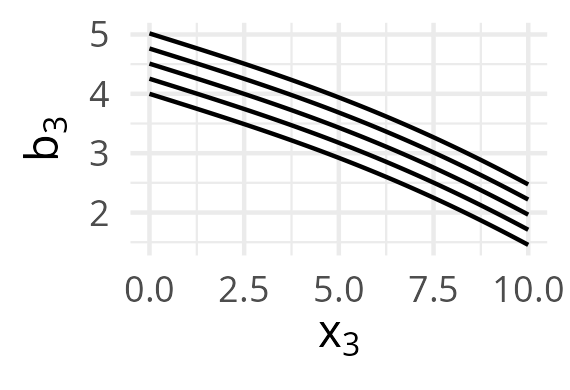
\includegraphics[width=\textwidth]{figure/boosting-cwb-blpool3.png}
  }{%
  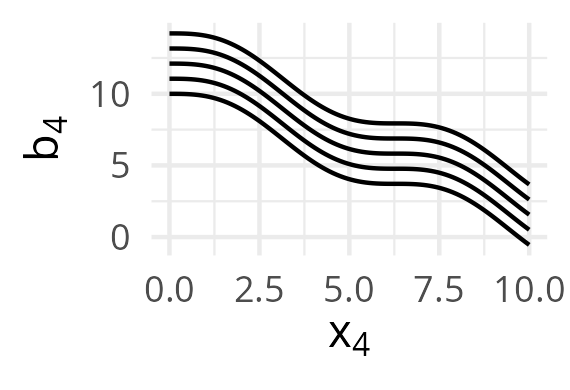
\includegraphics[width=\textwidth]{figure/boosting-cwb-blpool4.png}
  }
\end{frame}


% ------------------------------------------------------------------------------
% itemize wrapper
% ------------------------------------------------------------------------------

\begin{frame}{itemize wrappers}
  
  Presets fro \code{itemize} with different vertical spacings (\code{itemsep}). The default value for \code{itemsep} is apparently \code{2pt}. Use \code{\textbackslash the \textbackslash itemsep} to find out the current value.
  
  
  \vfill
  
  \splitVTT{
  \begin{itemize}
    \item \textbf{Default itemize}
    \item itemsep is unmodified
    \item Another thing
    \item Words
    \item A fourth thing to show
    \item Just filling space here
    \item Hello there
  \end{itemize}
  }{
  \begin{itemizeS}
    \item \textbf{Uses environment} \code{itemizeS}
    \item itemsep is: \the\itemsep
    \item Another thing
    \item Words
    \item A fourth thing to show
    \item Just filling space here
    \item Hello there
  \end{itemizeS}
  }
  
\end{frame}

% ------------------------------------------------------------------------------

\begin{frame}{itemizeM and itemizeL}
  
  \splitVTT{
  \begin{itemizeM}
    \item \textbf{Default itemize} with  \code{itemizeM}
    \item itemsep is unmodified
    \item Another thing
    \item Words
    \item A fourth thing to show
    \item Just filling space here
    \item Hello there
  \end{itemizeM}
  }{
  \begin{itemizeL}
    \item \textbf{Uses environment} \code{itemizeL}
    \item itemsep is: \the\itemsep
    \item Another thing
    \item Words
    \item A fourth thing to show
    \item Just filling space here
    \item Hello there
  \end{itemizeL}
  }
  
\end{frame}

% ------------------------------------------------------------------------------

\begin{frame}{itemizeF for vertical filling}
  \begin{itemizeF}
    \item \textbf{Uses environment} \code{itemizeF}
    \item itemsep is: \the\itemsep
    \item Automatically uses all vertical space
    \item Depends on containing enviornment though!
  \end{itemizeF}
\end{frame}

% ------------------------------------------------------------------------------

\begin{frame}{itemize Spacing and Font Size control}
  
  \begin{columns}[T]
    \begin{column}{0.48\textwidth}
      \textbf{itemizeS with small text}
      \begin{itemizeS}[small]
        \item Small font + compact spacing
        \item Use for detailed lists
        \item When every line matters
      \end{itemizeS}
    \end{column}
    
    \begin{column}{0.48\textwidth}
      \textbf{itemizeL with large text:}
      \begin{itemizeL}[large]
        \item Large font + wide spacing
        \item Makes content stand out
        \item Ideal for takeaways
      \end{itemizeL}
    \end{column}
  \end{columns}
  
  \vfill
  
  \textbf{itemizeM with default text:}
  \begin{itemizeM}
    \item Default sizing and spacing works best for most content
    \item Provides good readability and balanced slide appearance
  \end{itemizeM}

  \vfill

  \textbf{itemizeM with footnotesize text:}
  \begin{itemizeM}[footnotesize]
    \item Default sizing and spacing works best for most content
    \item Provides good readability and balanced slide appearance
  \end{itemizeM}
  
\end{frame}


% \begin{frame}{itemize Key-Value Interface}
%   \code{itemizeL} etc. buitl on \code{kitemize} environment with key-value interface:
  
%   \vspace{1ex}
%   \texttt{\\begin\{kitemize\}[fs=small,sep=S]}
%   \begin{kitemize}[fs=small,sep=S]
%     \item Font size: \texttt{fs=small}
%     \item Separation: \texttt{sep=S}
%     \item Both parameters are optional
%   \end{kitemize}
  
%   \vspace{1ex}
%   \texttt{\\begin\{kitemize\}[fs=large,sep=L]}
%   \begin{kitemize}[fs=large,sep=L]
%     \item Large font
%     \item Wide spacing
%     \item Better readability
%   \end{kitemize}
% \end{frame}

% ------------------------------------------------------------------------------
% image helpers
% ------------------------------------------------------------------------------

\begin{frame}{Image taking the full slide width}
  \image{figure_man/neo3_2.png}
\end{frame}

\begin{frame}{Image using half the available width}
  \image[0.5]{figure_man/neo3_2.png}
\end{frame}

\begin{frame}{Centered image using half the available width}
  \imageC[0.5]{figure_man/neo3_2.png}
\end{frame}


% ------------------------------------------------------------------------------

\begin{frame}{Full width centered image with attribution}
  \imageC[1][KITTEN]{figure_man/neo3_2.png}
\end{frame}

% ------------------------------------------------------------------------------

\begin{frame}{Images with alignment and attribution}
  
  \imageL[0.4][CITEKEY]{figure/gbm_sine.png}
  \imageC[0.4][CITEKEY]{figure/gbm_sine.png}
  \imageR[0.4][CITEKEY]{figure/gbm_sine.png}
  
\end{frame}

% ------------------------------------------------------------------------------

\begin{frame}{Images within itemize}
  
  \begin{itemize}
    \item Foo bar
    \item Plubber
    \imageC[0.5]{figure/boosting-cwb-blpool1.png}
    \item jfowiehfgnsdlkjnfg
  \end{itemize}
  
\end{frame}

% ------------------------------------------------------------------------------

\begin{frame}{Images within splitV}
  
  \splitVTT[0.4]{
  \image{figure/boosting-cwb-blpool1.png}
  }{
  \image{figure/boosting-cwb-blpool1.png}
  }
  
  \vfill
  
  \splitVCC[0.4]{
  \image{figure/boosting-cwb-blpool1.png}
  }{
  \image{figure/boosting-cwb-blpool1.png}
  }
  
\end{frame}

% ------------------------------------------------------------------------------

\begin{frame}{Images within splitVCC}
  
  \splitVCC{
  \image[0.5]{figure_man/neo3_2.png}
  }{
  \image[0.7]{figure_man/neo3_2.png}
  }
  
  \vfill
  
  \splitVCC[0.4]{
  \imageC[1][KITTEN]{figure_man/neo3_2.png}
  }{
  \image{figure_man/neo3_2.png}
  }
  
\end{frame}

% ------------------------------------------------------------------------------
% framei
% ------------------------------------------------------------------------------

\begin{framei}{framei environment}
  \item This is a frame consisting only of an itemize environment
  \item Nothing else here, just itemize.
  \item No extra options yet for alignment or sizing in this case
  \imageC[0.6]{figure_man/neo3_2.png}
  \item Look, an image
\end{framei}

% ------------------------------------------------------------------------------

\begin{framei}[fs=small,sep=S]{Customized framei Environment}
  \item The \texttt{framei} environment supports key-value arguments
  \item Font size: \texttt{fs=small} (or footnotesize, large, etc.)
  \item Separation: \texttt{sep=S} (or M, L, F)
  \item This example uses \texttt{framei[fs=small,sep=S]}
  \item Perfect for overview slides or detailed lists
  \item Makes it easy to fit more content on a single slide
  \item Please don't overdo it
\end{framei}

% ------------------------------------------------------------------------------

\begin{framei}[fs=large,sep=L]{Another framei Example}
  \item Larger text with wider spacing
  \item Passed directly to the \texttt{framei} environment
  \item Using \texttt{[fs=large,sep=L]}
  \item For emphasis and impact
\end{framei}

% ------------------------------------------------------------------------------

\begin{framei}[fs=large,sep=F]{A filling framei Example}
  \item Larger text with widest spacing
  \item Passed directly to the \texttt{framei} environment
  \item Using \texttt{[fs=large,sep=F]}
  \item For the glory of hypnotoad
\end{framei}

% ------------------------------------------------------------------------------

\begin{framei}[fs=footnotesize,sep=M]{Integration with framei Environment}
  \item The framei environment creates an itemize list
  \item We can nest splitV inside list items
  
  \item Using splitVTT within a list item:
  \splitVCC{
    \item This continues the itemize list
    \item No need for a nested itemize
    \item The items appear properly beside the image
  }{
    \imageC[1][KITTEN]{figure_man/neo3_3.png}
  }
  
  \item Back to the main list
  \item With proper spacing between elements
\end{framei}

% ------------------------------------------------------------------------------

\begin{frame}{SplitV Inside Regular Itemize}
  \begin{itemize}
    \item First regular bullet point
    
    \item In case of \textbf{complete separation}, optimization might fail
    \splitVCC[0.6]{
      \item This appears beside the image
      \item No need for a nested itemize environment
    }{
      \image[0.6]{figure_man/neo3_3.png}
    }
    
    \item Assume data is separable
    \item We can continue the list afterward
    
    \item Another example with top alignment:
    \splitVTT[0.7]{
      \item Top-aligned content
      \item In a normal itemize environment
    }{
      \image[0.8]{figure_man/neo3_1.png}
    }
    
    \item Final regular bullet point
  \end{itemize}
\end{frame}

% ------------------------------------------------------------------------------

\begin{frame2}[small]{frame2 like frame but with font size parameter}
  This entire frame uses the small font size.
  
  \begin{itemize}
    \item this regular itemize list uses the small font size
=    \item you can nest things in here as needed
  \end{itemize}
\end{frame2}

% ------------------------------------------------------------------------------

\endlecture
\end{document}
